\chapter{Specificatie}

Het te ontwikkelen systeem zal moeten voldoen aan de volgende functionele
specificaties:

\begin{itemize}
    \item Het systeem moet plug-n-play zijn;
    \item het systeem moet gemarkeerde doelen kunnen detecteren door middel van
        een camera;
    \item het systeem moet op de gedetecteerde doelen Nerf-darts (figuur
        \ref{fig:dart}) schieten;
    \item het systeem moet met minder dan optimaal omgevingslicht nog steeds
        naar behoren werken;
    \item het systeem moet op een embedded applicatie functioneren;
    \item het systeem moet verplaatsbaar zijn;
\end{itemize}

Een optionele eis is het toevoegen van kleur schiet-intensiteit door
bijvoorbeeld de kleur van de \emph{marker} te gebruiken (bijvoorbeeld rood
voor de hoogste intensiteit, orange voor een gemiddelde intensiteit en groen
voor een lage intensiteit).

\begin{figure}
    \begin{center}
        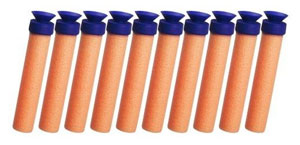
\includegraphics[scale=0.75]{figures/darts.jpg}
    \end{center}
    \caption{Een Nerf-dart}
    \label{fig:dart}
\end{figure}
